\documentclass[a4paper]{article}
\usepackage[a4paper,margin=0mm]{geometry}
\usepackage{fontspec}
\usepackage{unicode-math}
\usepackage{tikz}
\usepackage[table]{xcolor}
\usepackage[absolute]{textpos}
\usepackage{enumitem}
\usepackage{array}
\usepackage{multirow}

\setmainfont{Libertinus Serif}
\setsansfont{Libertinus Sans}
\setmathfont{Libertinus Math}
\newfontfamily\trackedsans{Libertinus Sans}[LetterSpace=8.0]

\definecolor{accent}{HTML}{F46530}
\definecolor{badge}{HTML}{FFBDA5}
\definecolor{ink}{HTML}{2A2E30}

\setlength{\TPHorizModule}{1mm}
\setlength{\TPVertModule}{1mm}
\setlength{\parindent}{0pt}
\pagestyle{empty}

\newcommand{\LCOL}{16mm}
\newcommand{\RCOL}{111mm}
\newcommand{\COLW}{83mm}

\newcommand{\topicheader}[2]{%
\begin{textblock*}{194mm}(16mm,10mm)
\begin{tikzpicture}
\node[fill=accent,text=white,font=\sffamily\bfseries\fontsize{13}{13}\selectfont,
      minimum width=9mm,minimum height=9mm,inner sep=0pt] at (4.5mm,-4.5mm) {#1};
\node[font=\sffamily\bfseries\fontsize{15}{16}\selectfont,text=ink,anchor=west] at (12mm,-4.5mm) {#2};
\end{tikzpicture}
\end{textblock*}
\begin{textblock*}{194mm}(16mm,22.5mm)

\begin{tikzpicture}
\fill[accent] (0,0) rectangle (194mm,0.5mm);
\end{tikzpicture}
\end{textblock*}
}

\newcommand{\pagefooter}[1]{%
\begin{textblock*}{194mm}(8mm,286.41mm)
  
\begin{tikzpicture}
    \fill[accent] (0,0) rectangle (194mm,0.6mm);
  \end{tikzpicture}
\end{textblock*}
\begin{textblock*}{63.59mm}(8mm,288.27mm)
  {\sffamily\bfseries\color{accent}\fontsize{13}{16}\selectfont SAT 1200+}
\end{textblock*}
\begin{textblock*}{10mm}(188mm,288.27mm)
  \centering{\sffamily\color{accent}\fontsize{14}{16}\selectfont #1}
\end{textblock*}
}

\newcommand{\colrule}[2]{%
\begin{textblock*}{1mm}(105mm,#1mm)
\begin{tikzpicture}
\draw[black!65,line width=0.5pt] (0,0) -- (0,#2mm);
\end{tikzpicture}
\end{textblock*}
}

\newcommand{\setkicker}[2]{%
{\sffamily\bfseries\fontsize{12}{14}\selectfont #1.}\ {\itshape\fontsize{11}{14}\selectfont\color{black!75} #2}\par\vspace{2mm}%
}

\setlength{\fboxsep}{1.4pt}
\setlength{\fboxrule}{0.5pt}
\newcommand{\pnum}[1]{\fcolorbox{ink}{white}{\sffamily\bfseries\fontsize{8}{8}\selectfont #1}~}

\newcommand{\qrbox}[1]{%
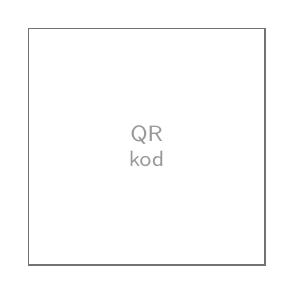
\begin{tikzpicture}
\draw[black!55,line width=0.6pt] (0,0) rectangle (30mm,30mm);
\node[black!40,font=\sffamily\fontsize{8}{9}\selectfont,align=center] at (15mm,15mm) {QR\\kod};
\end{tikzpicture}\\[1.5mm]
{\sffamily\fontsize{9}{11}\selectfont\color{black!70} #1}%
}

\arrayrulecolor{accent}
\setlength{\arrayrulewidth}{0.7pt}
\renewcommand{\arraystretch}{1.35}
\newcommand{\anstitle}[1]{{\sffamily\bfseries\color{accent}\fontsize{11}{13}\selectfont #1}\\[1.3mm]}

\begin{document}

% ================= PAGE 1: Set 1 | Set 2 =================
\topicheader{20}{Yuza va Hajm}
\pagefooter{1}
\colrule{32}{238}
\mbox{}%

\begin{textblock*}{\COLW}(\LCOL,32mm)
{\fontsize{11}{14}\selectfont
\setkicker{1-to'plam}{Asosiy maydon formulalari.}

\noindent\pnum{1} To'g'ri to'rtburchakning uzunligi $12$ sm, kengligi $5$ sm. Maydonini toping.\\[18mm]
\noindent\pnum{2} Uchburchakning asosi $14$ sm, balandligi $6$ sm. Maydonini toping.\\[18mm]
\noindent\pnum{3} Parallelogrammning asosi $9$ sm, balandligi $7$ sm. Maydonini toping.\\[18mm]
\noindent\pnum{4} Trapetsiyaning ikki asosi $5$ sm va $11$ sm, balandligi $8$ sm. Maydonini toping.\\[18mm]
\noindent\pnum{5} Doiraning radiusi $7$ sm. Maydonini toping.\\[18mm]
\noindent\pnum{6} Doiraning diametri $20$ sm. Maydonini toping.
}
\end{textblock*}

\begin{textblock*}{\COLW}(\RCOL,32mm)
{\fontsize{11}{14}\selectfont
\setkicker{2-to'plam}{Asosiy hajm formulalari.}

\noindent\pnum{1} To'g'ri burchakli prizmaning o'lchamlari $8$ sm, $5$ sm, $3$ sm. Hajmini toping.\\[18mm]
\noindent\pnum{2} Silindrning radiusi $4$ sm, balandligi $10$ sm. Hajmini toping.\\[18mm]
\noindent\pnum{3} Konusning radiusi $6$ sm, balandligi $9$ sm. Hajmini toping.\\[18mm]
\noindent\pnum{4} Sharning radiusi $3$ sm. Hajmini toping.\\[18mm]
\noindent\pnum{5} Silindrning diametri $10$ sm, balandligi $7$ sm. Hajmini toping.\\[18mm]
\noindent\pnum{6} Konusning diametri $8$ sm, balandligi $15$ sm. Hajmini toping.
}
\end{textblock*}

\clearpage

% ================= PAGE 2: Set 3 (addition) | Set 4 (subtraction) =================
\topicheader{20}{Yuza va Hajm}
\pagefooter{2}
\colrule{32}{238}
\mbox{}%

\begin{textblock*}{\COLW}(\LCOL,32mm)
{\fontsize{10.5}{13.5}\selectfont
\setkicker{3-to'plam}{Qo'shma figuralar -- qo'shish, hech narsa kesib olinmagan.}

\noindent\pnum{1} ``L'' shaklidagi figura ikki to'g'ri to'rtburchakdan iborat: $10$ sm $\times$ $6$ sm va unga yopishtirilgan $4$ sm $\times$ $3$ sm. Umumiy maydonni toping.\\[14mm]
\noindent\pnum{2} To'g'ri to'rtburchak $8$ sm $\times$ $5$ sm, uning tepasiga asosi $8$ sm, balandligi $4$ sm bo'lgan uchburchak qo'shilgan (uy tomi shaklida). Umumiy maydonni toping.\\[14mm]
\noindent\pnum{3} To'g'ri to'rtburchak $10$ sm $\times$ $6$ sm, uning uzun tomoniga radiusi $5$ sm bo'lgan yarim doira qo'shilgan. Umumiy maydonni toping.\\[14mm]
\noindent\pnum{4} Ikki to'g'ri burchakli prizma birlashtirilgan: birinchisi $10\times4\times3$ sm, ikkinchisi $4\times4\times6$ sm. Umumiy hajmni toping.\\[14mm]
\noindent\pnum{5} Tomoni $9$ sm bo'lgan kvadratga, kateti $6$ sm va $8$ sm bo'lgan to'g'ri burchakli uchburchak qo'shilgan. Umumiy maydonni toping.\\[14mm]
\noindent\pnum{6} Radiusi $3$ sm, balandligi $10$ sm bo'lgan silindrning ustiga xuddi shu radiusli, balandligi $4$ sm bo'lgan konus qo'yilgan. Umumiy hajmni toping.
}
\end{textblock*}

\begin{textblock*}{\COLW}(\RCOL,32mm)
{\fontsize{10.5}{13.5}\selectfont
\setkicker{4-to'plam}{Qo'shma figuralar -- ayirish, bir qism kesib olingan.}

\noindent\pnum{1} Tomoni $10$ sm bo'lgan kvadratning ichidan radiusi $3$ sm bo'lgan doira shaklida teshik kesib olingan. Qolgan maydonni toping.\\[14mm]
\noindent\pnum{2} To'g'ri to'rtburchak $12$ sm $\times$ $8$ sm. Uning ichidan tomoni $3$ sm bo'lgan kvadrat kesib olingan. Qolgan maydonni toping.\\[14mm]
\noindent\pnum{3} Radiusi $10$ sm bo'lgan katta doiraning ichida, xuddi shu markazda radiusi $4$ sm bo'lgan kichik doira teshik qilib olingan. Qolgan maydonni toping.\\[14mm]
\noindent\pnum{4} To'g'ri burchakli prizma $10\times8\times5$ sm. Uning ichidan $4\times3\times5$ sm o'lchamli bo'shliq kesib olingan. Qolgan hajmni toping.\\[14mm]
\noindent\pnum{5} Ikki asosi $10$ sm va $16$ sm, balandligi $8$ sm bo'lgan trapetsiyadan, asosi $4$ sm va balandligi $6$ sm bo'lgan uchburchak kesib olingan. Qolgan maydonni toping.\\[14mm]
\noindent\pnum{6} Radiusi $5$ sm, balandligi $12$ sm bo'lgan silindrning ichidan, xuddi shu radius va balandlikka ega konus shaklidagi bo'shliq o'yib olingan. Qolgan hajmni toping.
}
\end{textblock*}

\clearpage

% ================= PAGE 3: Set 5 (missing dimension) | Set 6 (spot the error) =================
\topicheader{20}{Yuza va Hajm}
\pagefooter{3}
\colrule{32}{238}
\mbox{}%

\begin{textblock*}{\COLW}(\LCOL,32mm)
{\fontsize{11}{14}\selectfont
\setkicker{5-to'plam}{Teskari yo'nalish -- maydon/hajm berilgan, o'lchamni toping.}

\noindent\pnum{1} To'g'ri to'rtburchakning maydoni $72$ sm$^2$, kengligi $8$ sm. Uzunligini toping.\\[18mm]
\noindent\pnum{2} Uchburchakning maydoni $35$ sm$^2$, asosi $10$ sm. Balandligini toping.\\[18mm]
\noindent\pnum{3} Doiraning maydoni $81\pi$ sm$^2$. Doiraning diametrini toping.\\[18mm]
\noindent\pnum{4} To'g'ri burchakli prizmaning hajmi $200$ sm$^3$, uzunligi $10$ sm, kengligi $4$ sm. Balandligini toping.\\[18mm]
\noindent\pnum{5} Silindrning hajmi $250\pi$ sm$^3$, radiusi $5$ sm. Balandligini toping.\\[18mm]
\noindent\pnum{6} Sharning hajmi $288\pi$ sm$^3$. Sharning radiusini toping.
}
\end{textblock*}

\begin{textblock*}{\COLW}(\RCOL,32mm)
{\fontsize{10}{13}\selectfont
\setkicker{6-to'plam}{Xatoni toping -- buzilgan qoidani ayting, to'g'ri javobni bering.}

\noindent\pnum{1} ``Doiraning diametri $10$ sm. Maydonini toping.'' ifodasida ko'rsatilgan yechimda xato bor:\\[1mm]
\hspace*{7mm}\textit{``$A=\pi(10)^2=100\pi$.''}\\[2mm]
\hspace*{7mm}Xato va to'g'ri javob: \makebox[52mm]{\dotfill}\\[6mm]

\noindent\pnum{2} ``Tomoni $8$ sm bo'lgan kvadratning ichida radiusi $2$ sm bo'lgan doira teshik bor. Qolgan maydonni toping.'' ifodasida ko'rsatilgan yechimda xato bor:\\[1mm]
\hspace*{7mm}\textit{``$64+4\pi$.''}\\[2mm]
\hspace*{7mm}Xato va to'g'ri javob: \makebox[52mm]{\dotfill}\\[6mm]

\noindent\pnum{3} ``Konusning radiusi $3$ sm, balandligi $10$ sm. Hajmini toping.'' ifodasida ko'rsatilgan yechimda xato bor:\\[1mm]
\hspace*{7mm}\textit{``$V=\pi(3)^2(10)=90\pi$.''}\\[2mm]
\hspace*{7mm}Xato va to'g'ri javob: \makebox[52mm]{\dotfill}\\[6mm]

\noindent\pnum{4} ``Sharning radiusi $5$ sm. Hajmini toping.'' ifodasida ko'rsatilgan yechimda xato bor:\\[1mm]
\hspace*{7mm}\textit{``$V=\pi(5)^3=125\pi$.''}\\[2mm]
\hspace*{7mm}Xato va to'g'ri javob: \makebox[52mm]{\dotfill}\\[6mm]

\noindent\pnum{5} ``Silindrning diametri $6$ sm, balandligi $10$ sm. Hajmini toping.'' ifodasida ko'rsatilgan yechimda xato bor:\\[1mm]
\hspace*{7mm}\textit{``$V=\pi(6)^2(10)=360\pi$.''}\\[2mm]
\hspace*{7mm}Xato va to'g'ri javob: \makebox[52mm]{\dotfill}
}
\end{textblock*}

\clearpage

% ================= PAGE 4: Set 7 (bonus) -- own page =================
\topicheader{20}{Yuza va Hajm}
\pagefooter{4}
\colrule{32}{238}
\mbox{}%

\begin{textblock*}{\COLW}(\LCOL,32mm)
{\fontsize{10.5}{13.5}\selectfont
\setkicker{7-to'plam}{Bonus / qiyin -- ko'p bosqichli masalalar.}

\noindent\pnum{1} To'g'ri burchakli prizma $10\times10\times20$ sm. Uning ichidan, balandligi bo'ylab o'tadigan radiusi $2$ sm bo'lgan silindrik teshik kesib olingan. Qolgan hajmni toping.\\[24mm]
\noindent\pnum{2} Tomoni $14$ sm bo'lgan kvadratdan, radiusi $7$ sm bo'lgan bitta to'liq doira shaklida qism kesib olingan. Qolgan maydonni toping.\\[24mm]
\noindent\pnum{3} Radiusi $4$ sm, balandligi $10$ sm bo'lgan silindrning ustiga, xuddi shu radiusli yarim shar joylashtirilgan. Umumiy hajmni toping.
}
\end{textblock*}

\begin{textblock*}{\COLW}(\RCOL,32mm)
{\fontsize{10.5}{13.5}\selectfont
\vspace*{0mm}
\noindent\pnum{4} Ko'ndalang kesimi trapetsiya shaklida bo'lgan prizma: trapetsiyaning asoslari $6$ sm va $10$ sm, balandligi $4$ sm; prizmaning uzunligi $15$ sm. Prizmaning hajmini toping.\\[24mm]
\noindent\pnum{5} Radiusi $6$ sm, balandligi $15$ sm bo'lgan silindrning ichidan, xuddi shu radius va balandlikka ega konus shaklidagi bo'shliq olib tashlangan. Qolgan hajmni toping.
}
\end{textblock*}

\clearpage

% ================= PAGE 5: Javoblar =================
\topicheader{20}{Yuza va Hajm}
\pagefooter{5}
\mbox{}%

\begin{textblock*}{194mm}(16mm,30mm)
{\bfseries\itshape\color{accent}\fontsize{19}{21}\selectfont\centering Javoblar\par}
\end{textblock*}

\begin{textblock*}{194mm}(16mm,44mm)
{\fontsize{9}{11.5}\selectfont
\centering
\renewcommand{\arraystretch}{1.3}
\begin{tabular}{|>{\centering\arraybackslash}p{22mm}|>{\centering\arraybackslash}p{9mm}|>{\centering\arraybackslash}p{30mm}|>{\centering\arraybackslash}p{9mm}|>{\centering\arraybackslash}p{30mm}|}
\hline
\rowcolor{badge!55}\textbf{To'plam} & \textbf{\#} & \textbf{Javob} & \textbf{\#} & \textbf{Javob}\\
\hline
\multirow{3}{22mm}{\centering 1-to'plam} & 1 & $60$ sm$^2$ & 2 & $42$ sm$^2$\\\cline{2-5}
 & 3 & $63$ sm$^2$ & 4 & $64$ sm$^2$\\\cline{2-5}
 & 5 & $49\pi$ sm$^2$ & 6 & $100\pi$ sm$^2$\\\hline
\multirow{3}{22mm}{\centering 2-to'plam} & 1 & $120$ sm$^3$ & 2 & $160\pi$ sm$^3$\\\cline{2-5}
 & 3 & $108\pi$ sm$^3$ & 4 & $36\pi$ sm$^3$\\\cline{2-5}
 & 5 & $175\pi$ sm$^3$ & 6 & $80\pi$ sm$^3$\\\hline
\multirow{3}{22mm}{\centering 3-to'plam} & 1 & $72$ sm$^2$ & 2 & $56$ sm$^2$\\\cline{2-5}
 & 3 & $60+\frac{25}{2}\pi$ sm$^2$ & 4 & $216$ sm$^3$\\\cline{2-5}
 & 5 & $105$ sm$^2$ & 6 & $102\pi$ sm$^3$\\\hline
\multirow{3}{22mm}{\centering 4-to'plam} & 1 & $100-9\pi$ sm$^2$ & 2 & $87$ sm$^2$\\\cline{2-5}
 & 3 & $84\pi$ sm$^2$ & 4 & $340$ sm$^3$\\\cline{2-5}
 & 5 & $92$ sm$^2$ & 6 & $200\pi$ sm$^3$\\\hline
\multirow{3}{22mm}{\centering 5-to'plam} & 1 & $l=9$ sm & 2 & $h=7$ sm\\\cline{2-5}
 & 3 & $d=18$ sm & 4 & $h=5$ sm\\\cline{2-5}
 & 5 & $h=10$ sm & 6 & $r=6$ sm\\\hline
\multirow{2}{22mm}{\centering 7-to'plam} & 1 & $2000-80\pi$ sm$^3$ & 2 & $196-49\pi$ sm$^2$\\\cline{2-5}
 & 3 & $\frac{608}{3}\pi$ sm$^3$ & 4 & $480$ sm$^3$\\\cline{2-5}
 & 5 & \multicolumn{3}{p{70mm}|}{$360\pi$ sm$^3$}\\\hline
\multirow{5}{22mm}{\centering 6-to'plam} & \multicolumn{4}{p{72mm}|}{1.\ Diametrni radius o'rniga qo'ygan. To'g'ri: $r=5$, $A=\pi(5)^2=25\pi$.}\\\cline{2-5}
 & \multicolumn{4}{p{72mm}|}{2.\ Teshikni qo'shgan, ayirish kerak edi. To'g'ri: $64-4\pi$.}\\\cline{2-5}
 & \multicolumn{4}{p{72mm}|}{3.\ Konus koeffitsiyenti $\frac13$ unutilgan. To'g'ri: $\frac13\pi(3)^2(10)=30\pi$.}\\\cline{2-5}
 & \multicolumn{4}{p{72mm}|}{4.\ Shar koeffitsiyenti $\frac43$ unutilgan. To'g'ri: $\frac43\pi(5)^3=\frac{500}{3}\pi$.}\\\cline{2-5}
 & \multicolumn{4}{p{72mm}|}{5.\ Diametrni radius o'rniga qo'ygan. To'g'ri: $\pi(3)^2(10)=90\pi$.}\\\hline
\end{tabular}
}
\end{textblock*}

\begin{textblock*}{194mm}(16mm,240mm)
\centering
{\sffamily\fontsize{9.5}{11.5}\selectfont\color{black!70} Video yechimlar va qo'shimcha testlar uchun quyidagi QR kodlarni skanerlang:}\\[4mm]
\begin{minipage}[t]{32mm}\centering\qrbox{YouTube}\end{minipage}%
\hspace{16mm}%
\begin{minipage}[t]{32mm}\centering\qrbox{Telegram}\end{minipage}
\end{textblock*}

\end{document}
